  \ac{RIA} ist kein Standard, sondern ein synonym für Applikationen, welche
  eine ``reihhaltige'' Benutzeroberfläche bieten und eine Verbindung mit dem
  Internet haben.
  
  \section{Grundlagen}
  
  Der Begriff \ac{RIA} ist mit der Entwicklung des Internets entstanden und
  wird heute oft verwendet. Im Technologiespektrum steht die \ac{RIA} zwischen
  dem Rich Client und dem Thin Client, siehe Grafik \ref{img:webanwendungen}.
  
  \begin{figure}[h]
    \begin{center}
      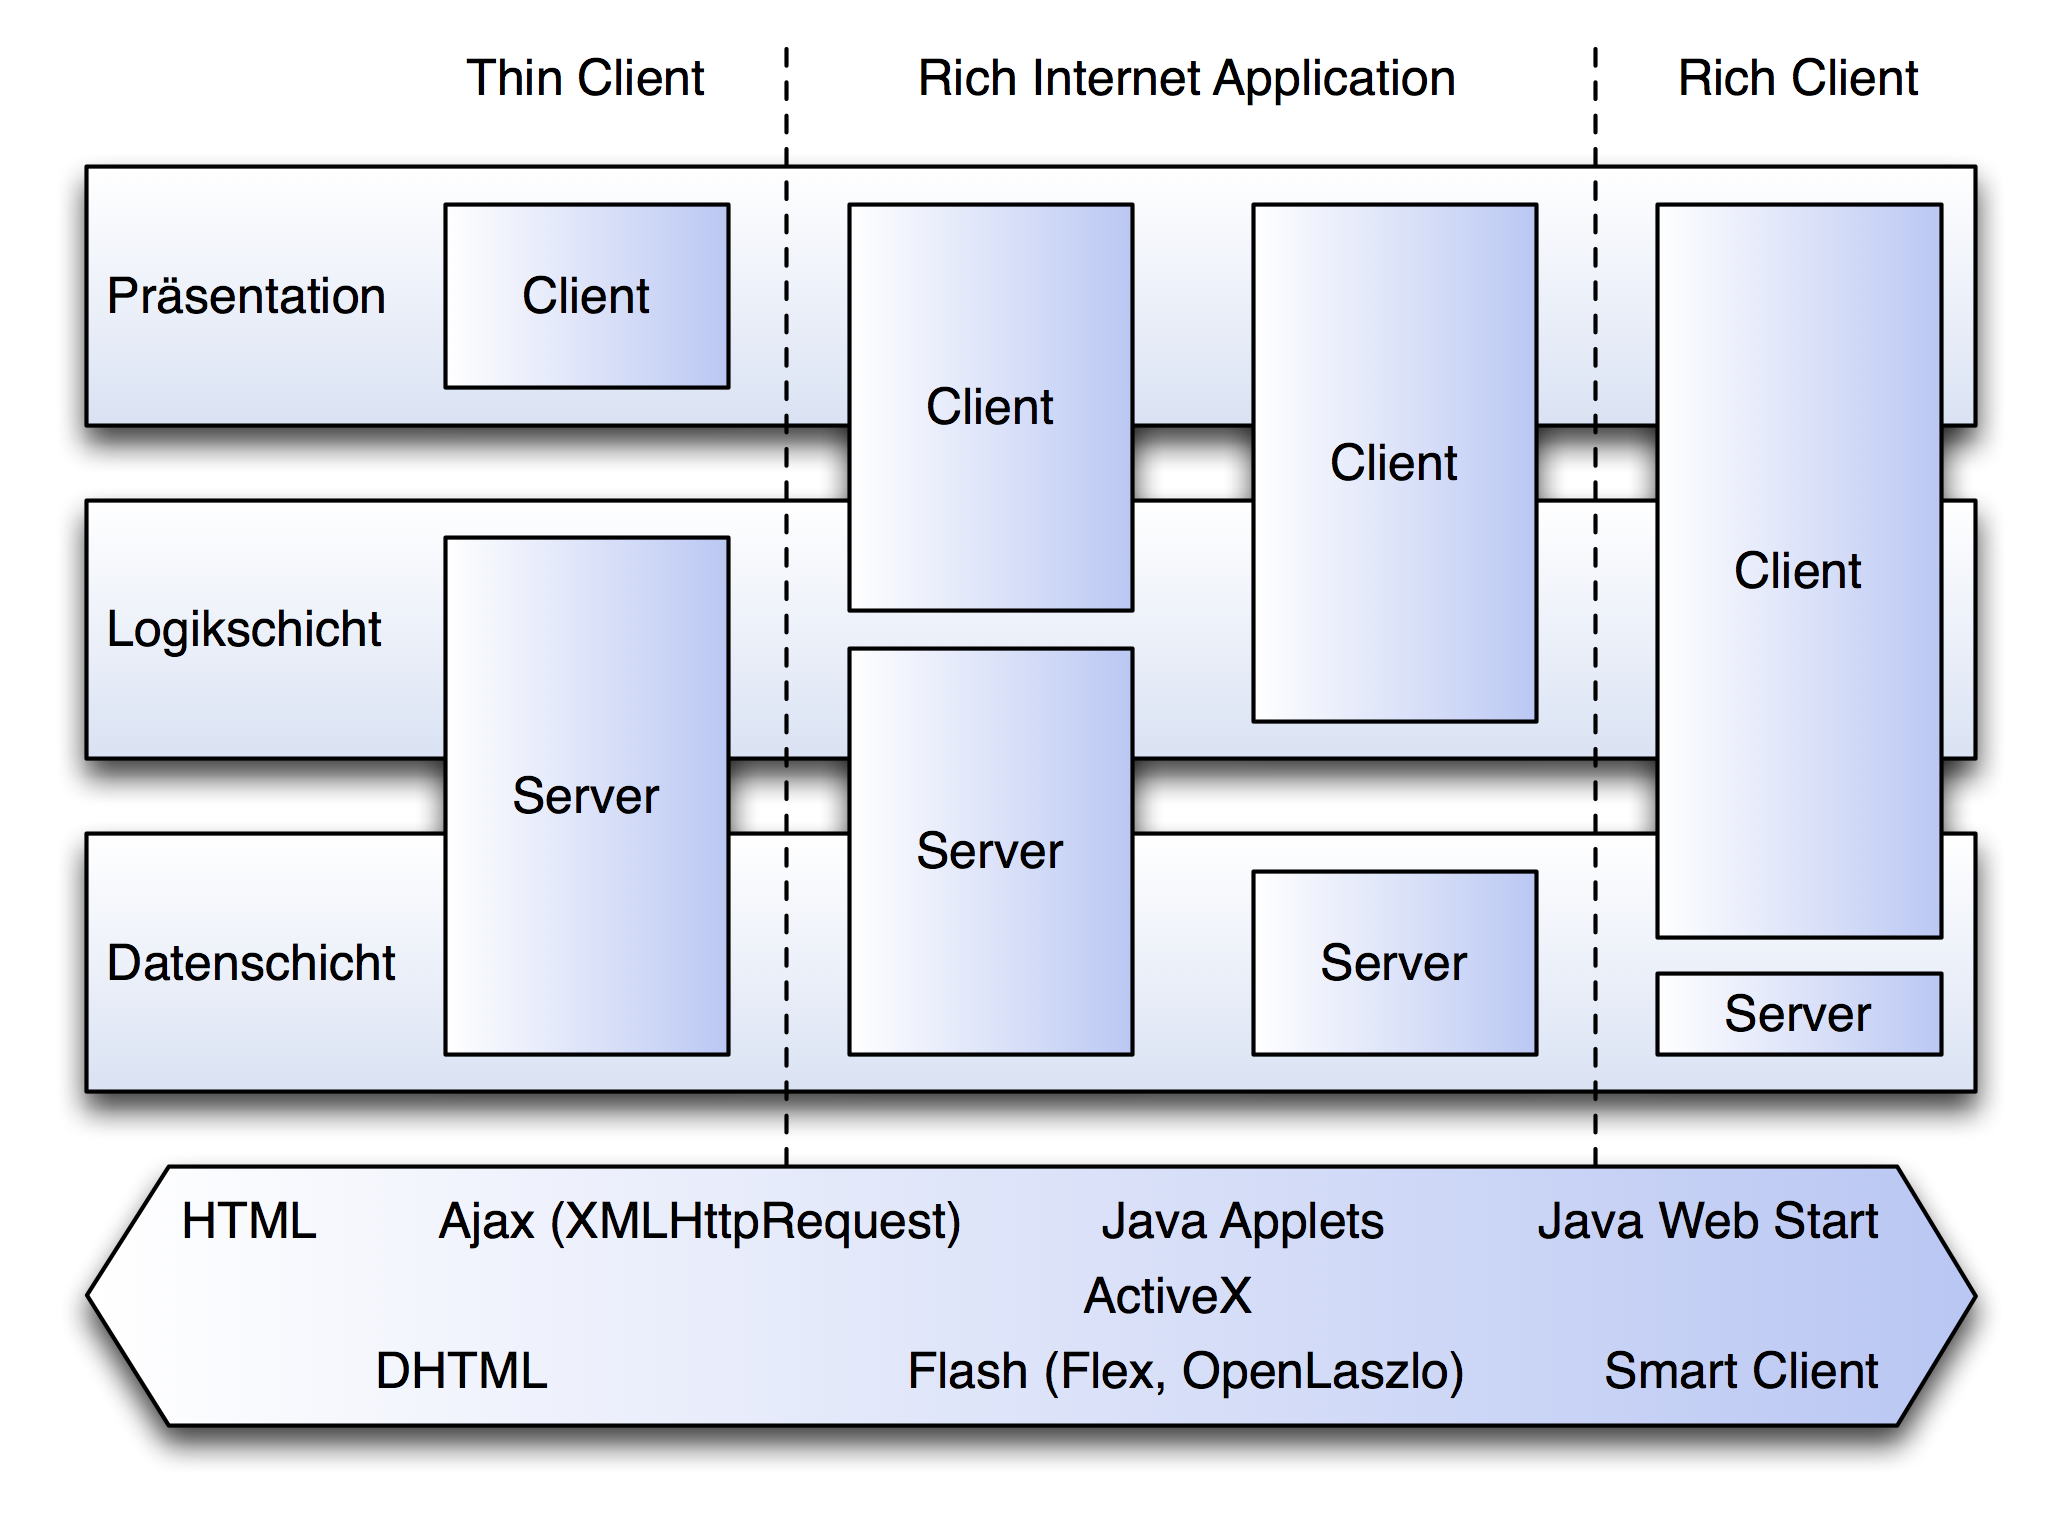
\includegraphics[width=0.7\textwidth]{./image/webanwendungen.png}
      \caption{Technologiespektrum von Web Anwendungen
      \cite{WebApplicationSolutions}}
      \label{img:webanwendungen}
    \end{center}
  \end{figure}
  
  
  \subsection{Client orientiert}

  \subsection{Browser orientiert}
  
  \subsection{Plugin orientiert}
  
  \section{Technologien}
  
  \subsection{Eingesetzte Standards}
  
  \subsection{Programmiermodell}
  
  \section{Security}
  
  \section{Merkmale}
    
  \subsection{Suchmaschinenoptimierung}
  
  \subsection{Barrierefreiheit}